% $Header: /Users/joseph/Documents/LaTeX/beamer/solutions/conference-talks/conference-ornate-20min.en.tex,v 90e850259b8b 2007/01/28 20:48:30 tantau $

\documentclass[xcolor={usenames,dvipsnames}]{beamer}

% This file is a solution template for:

% - Talk at a conference/colloquium.
% - Talk length is about 20min.
% - Style is ornate.



% Copyright 2004 by Till Tantau <tantau@users.sourceforge.net>.
%
% In principle, this file can be redistributed and/or modified under
% the terms of the GNU Public License, version 2.
%
% However, this file is supposed to be a template to be modified
% for your own needs. For this reason, if you use this file as a
% template and not specifically distribute it as part of a another
% package/program, I grant the extra permission to freely copy and
% modify this file as you see fit and even to delete this copyright
% notice. 


\mode<presentation>
{
  \usetheme{AnnArbor}
  % or ...

  \setbeamercovered{transparent}
  % or whatever (possibly just delete it)
 }

\usepackage[percent]{overpic}
\usepackage[english]{babel}
\usepackage{setspace}
% or whatever

\usepackage[latin1]{inputenc}
% or whatever

\usepackage[at]{easylist}
\usepackage{times}
\usepackage[T1]{fontenc}
\usepackage{xcolor}
% Or whatever. Note that the encoding and the font should match. If T1
% does not look nice, try deleting the line with the fontenc.

\definecolor{darkestblue}{RGB}{1,8,100}
\definecolor{darkerblue}{RGB}{3,17,150}
\definecolor{darkblue}{RGB}{7,26,200}
\definecolor{lightred}{RGB}{202,103,104}
\definecolor{lightgreen}{RGB}{106,202,107}

%particles
\newcommand{\jpsi}{\rm J/$\psi$}
\newcommand{\psip}{$\psi^\prime$}
\newcommand{\jpsiDY}{\rm J/$\psi$\,/\,DY}
\newcommand{\chic}{$\chi_{\rm c}$}
\newcommand{\pip}{$\pi^{+}$}
\newcommand{\pim}{$\pi^{-}$}
\newcommand{\pizero}{$\pi^{0}$}
\newcommand{\kap}{K$^{+}$}
\newcommand{\kam}{K$^{-}$}
\newcommand{\pbar}{$\rm\overline{p}$}
\newcommand{\ccbar}{\ensuremath{\mathrm{c\overline{c}}}}
\newcommand{\bbbar}{\ensuremath{\mathrm{b\overline{b}}}}
\newcommand{\Dzero}{\ensuremath{\mathrm{D^{0}}}}
\newcommand{\Dzerobar}{\ensuremath{\mathrm{\overline{D}^{0}}}}
\newcommand{\Dpm}{\ensuremath{\mathrm{D^{\pm}}}}
\newcommand{\Ds}{\ensuremath{\mathrm{D_{s}^{\pm}}}}
\newcommand{\Dstar}{\ensuremath{\mathrm{D^{*\pm}}}}

%collision systems
\newcommand{\pp}{pp}
\newcommand{\pPb}{p--Pb}
\newcommand{\PbPb}{Pb--Pb}

%detectors
\newcommand{\ezdc}{$E_{\rm ZDC}$}

%units
\newcommand{\GeVc}{GeV/$c$}
\newcommand{\GeVcsq}{GeV/$c^2$}

%others
\newcommand{\degree}{$^{\rm o}$}
\newcommand{\s}{\ensuremath{\sqrt{s}}}
\newcommand{\snn}{\ensuremath{\sqrt{s_{\rm NN}}}}
\newcommand{\y}{\ensuremath{y}}
\newcommand{\pt}{\ensuremath{p_{\rm T}}}
\newcommand{\dedx}{d$E$/d$x$}
\newcommand{\dndy}{d$N$/d$y$}
\newcommand{\dndydpt}{${\rm d}^2N/({\rm d}y {\rm d}p_{\rm t})$}
\newcommand{\zpar}{\ensuremath{z_{||}}}
\newcommand{\zpargen}{\ensuremath{z_{||}^{\mathrm{part}}}}
\newcommand{\zpardet}{\ensuremath{z_{||}^{\mathrm{det}}}}
\newcommand{\ptchjet}{\ensuremath{p_{\mathrm{T,ch\, jet}}}}
\newcommand{\ptjet}{\ensuremath{p_{\mathrm{T,jet}}}}
\newcommand{\ptchjetgen}{\ensuremath{p_{\mathrm{T,ch\,jet}}^{\mathrm{part}}}}
\newcommand{\ptchjetdet}{\ensuremath{p_{\mathrm{T,ch\,jet}}^{\mathrm{det}}}}
\newcommand{\ptd}{\ensuremath{p_{\mathrm{T,D}}}}
\newcommand{\ptdgen}{\ensuremath{p_{\mathrm{T,D}}^{\mathrm{part}}}}
\newcommand{\ptddet}{\ensuremath{p_{\mathrm{T,D}}^{\mathrm{det}}}}
\newcommand{\antikt}{anti-\ensuremath{k_{\mathrm{T}}}}
\newcommand{\Antikt}{Anti-\ensuremath{k_{\mathrm{T}}}}
\newcommand{\kt}{\ensuremath{k_{\mathrm{T}}}}
\newcommand{\pthard}{\ensuremath{p_{\mathrm{T,hard}}}}

\AtBeginSection[]{
  \begin{frame}
  \vfill
  \centering
  \begin{beamercolorbox}[sep=8pt,center,shadow=true,rounded=true]{title}
    \usebeamerfont{title}\insertsectionhead\par%
  \end{beamercolorbox}
  \vfill
  \end{frame}
}

\title[D-meson jets reconstruction with ALICE] % (optional, use only with long paper titles)
{D-meson jets reconstruction with ALICE}

\author[Salvatore Aiola]% (optional, use only with lots of authors)
{\underline{Salvatore Aiola} \\
PAG-HFCJ\\
PWG-HF}
% - Give the names in the same order as the appear in the paper.
% - Use the \inst{?} command only if the authors have different
%   affiliation.

\institute[Yale University] % (optional, but mostly needed)
{Yale University}

\date[July 27th, 2017] % (optional, should be abbreviation of conference name)
{Juniors' Day \\
ALICE Week \\
CERN, July 27th, 2017}
% - Either use conference name or its abbreviation.
% - Not really informative to the audience, more for people (including
%   yourself) who are reading the slides online

\subject{High-Energy Physics}
% This is only inserted into the PDF information catalog. Can be left
% out. 



% If you have a file called "university-logo-filename.xxx", where xxx
% is a graphic format that can be processed by latex or pdflatex,
% resp., then you can add a logo as follows:

% \pgfdeclareimage[height=0.5cm]{university-logo}{university-logo-filename}
% \logo{\pgfuseimage{university-logo}}


% If you wish to uncover everything in a step-wise fashion, uncomment
% the following command: 

%\beamerdefaultoverlayspecification{<+->}


\begin{document}

\begin{frame}
  \titlepage
\end{frame}

\begin{frame}{Outline}
   \tableofcontents
\end{frame}


% Structuring a talk is a difficult task and the following structure
% may not be suitable. Here are some rules that apply for this
% solution: 

% - Exactly two or three sections (other than the summary).
% - At *most* three subsections per section.
% - Talk about 30s to 2min per frame. So there should be between about
%   15 and 30 frames, all told.

% - A conference audience is likely to know very little of what you
%   are going to talk about. So *simplify*!
% - In a 20min talk, getting the main ideas across is hard
%   enough. Leave out details, even if it means being less precise than
%   you think necessary.
% - If you omit details that are vital to the proof/implementation,
%   just say so once. Everybody will be happy with that.


%\begin{overpic}[width=\textwidth, trim=0 0 0 0, clip]{img/823_D0_Charged_R040_JetPtBins_DPt_30}
%\end{overpic}

%\begin{columns}
%\column{0.5\textwidth}
%\column{0.5\textwidth}
%\end{columns}

\section{Introduction}

\subsection{Physics Motivations}
\begin{frame}[fragile]{Physics Motivations}
\begin{columns}
\column{0.70\textwidth}
\small
\begin{easylist}[itemize]
@ \pp\ collisions: improve quantitative comparisons with perturbative \textbf{\textcolor{ForestGreen}{Quantum Chromo-Dynamics}} (pQCD)
@@ $m_{\rm c} \sim 1$~\GeVcsq $\rightarrow$ pQCD valid down to $\pt\sim0$
@ \PbPb\ collisions: probe of the \textbf{\textcolor{BrickRed}{Quark-Gluon Plasma}} (QGP)
@@ Dynamics of the parton-medium interactions different for massless (u, d, s, g) vs.~massive (c, b) partons
@@ Parton mass effects significant only at low momenta
@ Relevant also to other fields: total charm cross section needed to calculate background for \textbf{\textcolor{NavyBlue}{high-energy neutrino astrophysics}}
\end{easylist}
\column{0.30\textwidth}
\begin{overpic}[width=\textwidth, trim=0 0 0 0, clip]{img/ALICE_D0Meson}
\end{overpic} \\
\vspace{5pt}
\begin{overpic}[width=\textwidth, trim=0 0 0 0, clip]{img/ALICE_DMesonRAA}
\end{overpic}
\end{columns}
\end{frame}

\subsection{Analysis Strategy}
\begin{frame}[fragile]{D-Tagged Jets With ALICE}
\begin{easylist}
@ \Dzero\ via \alert{hadronic decay}: $\Dzero\rightarrow{\rm K}^{\pm}\pi^{\mp}$ (B.R. 3.93\%)
@@ candidates identified among \alert{opposite-charge} track pairs
@@ combinatorial background reduced via
@@@ \alert{Particle Identification} (PID) on the decay products (\dedx\ and Time-Of-Flight)
@@@ \alert{topological cuts} on the secondary vertex ($c\tau=123\,\mu{\rm m}$)
@@ \alert{invariant mass analysis} to extract signal out of the residual combinatorial background
@ Jets reconstructed using \Dzero\ candidates and all other tracks
@@ \alert{\antikt} jet reconstruction algorithm (default choice at LHC)
@@ \alert{underlying event} (UE) subtracted using the jet areas (\PbPb\ only)
\end{easylist}
\end{frame}

\begin{frame}[fragile,t]{D-Tagged Jets With ALICE (cont'd)}
\begin{easylist}
@ Corrections
@@ \alert{Reconstruction efficiency} $\epsilon(\ptd)\approx5-25$\%
@@ \alert{Feed-Down} (FD) from B mesons $\sim10-30$\%
@@ \alert{Jet momentum resolution} $\sigma(\ptchjet)\approx 11$\%
\end{easylist}
\vspace{5pt}
N.B.: numbers above for \pp\ collisions
\end{frame}

\section{Preliminary Results}

\subsection{Detector Performance}

\begin{frame}{Efficiency and Resolution}
\begin{columns}
\column{.50\textwidth}
\centering
\textbf{Reconstruction Efficiency}\\
\vspace{2pt}
\begin{overpic}[width=\textwidth, trim=0 0 38 15, clip]{img/HQ16_Simulation_EfficiencyVsDPt}
\end{overpic}
\vspace{-15pt}
\begin{itemize}
\item \alert{Strong increase with \ptd} \\
$\rightarrow$ tighter topological cuts at low \ptd\
\item \textcolor{ForestGreen}{No dependence on \ptchjet}
\end{itemize}
\column{.50\textwidth}

\centering
\textbf{\ptchjet\ resolution} \\
\vspace{2pt}
\begin{overpic}[width=\textwidth, trim=0 0 38 15, clip]{img/HQ16_Simulation_Resolution}
\end{overpic}
\vspace{-15pt}
\begin{itemize}
\item \ptchjet\ resolution dominated by \alert{tracking efficiency}
\item \alert{No \pt\ dependence} in the range $5<\ptchjet<24$ \GeVc
\end{itemize}
\end{columns}
\end{frame}

\subsection{Results}

\begin{frame}{Raw Signal Extraction}
\centering
\begin{overpic}[width=0.73\textwidth, trim=0 0 0 0 0, clip]{img/SideBandInvMass_QM17}
\end{overpic}
\footnotesize
\begin{itemize}
\item \textbf{\textcolor{darkestblue}{Invariant mass distributions}} of identified \Dzero-jet candidates are \textbf{\textcolor{darkblue}{fit}} with a Guassian + exponential $\rightarrow$ peak position \& width, background normalization
\item The \ptchjet\ distributions of the \textbf{\textcolor{lightgreen}{side bands}} are subtracted from those of the \textbf{\textcolor{lightred}{signal region}} and weighted by the efficiency $\epsilon_{\Dzero}(\ptd)$ % (Fig.~\ref{fig:HQ16_Simulation_EfficiencyVsDP})
\end{itemize}
\centering
 $\textcolor{darkerblue}{N(\ptchjet)}=\sum_{\ptd}\frac{1}{\epsilon_{\Dzero}(\ptd)} \cdot \left[\textcolor{lightred}{N_{\rm Sign}(\ptd,\ptchjet)}-B'\textcolor{lightgreen}{N_{\rm SB}(\ptd,\ptchjet)} \right]$
\end{frame}

\begin{frame}{B Feed-Down ($\rm B\rightarrow$\Dzero)}
\begin{columns}
\column{.50\textwidth}
\begin{overpic}[width=\textwidth, trim=0 0 0 0 0, clip]{img/Efficiency_QM17}
\end{overpic}
\column{.50\textwidth}
\begin{overpic}[width=\textwidth, trim=0 0 0 0 0, clip]{img/BFeedDown_QM17}
\end{overpic}
\end{columns}
\begin{description}
\item[Prompt:]\hspace{2pt} fragmentation of a c quark 
\item[Non-Prompt:]\hspace{2pt} decay of a B hadron
\end{description}
Due to the longer decay length of the B hadrons, the topological cuts are more efficient for non-prompt \Dzero, thus biasing the
relative contributions. We subtract the B feed-down fraction using POWHEG+PYTHIA6.
\end{frame}

\begin{frame}{Unfolding (jet \pt\ resolution)}
\begin{columns}
\column{.50\textwidth}
\begin{center}
\tiny
Method Comparison
\begin{overpic}[width=.8\textwidth, trim=0 0 0 0, clip]{img/SideBand_DPt_30_UnfoldingMethod_Ratio}
\end{overpic}\\
Bayesian Regularization
\begin{overpic}[width=.8\textwidth, trim=0 0 0 0, clip]{img/SideBand_DPt_30_UnfoldingRegularization_Bayes_PriorResponseTruth_Ratio}
\end{overpic}
\end{center}
\column{.50\textwidth}
\begin{center}
\tiny
Prior Choice \\
\begin{overpic}[width=.8\textwidth, trim=0 0 0 0, clip]{img/SideBand_DPt_30_UnfoldingPrior_Bayes_Ratio}
\end{overpic}
\end{center}
\vspace{-20pt}
\begin{itemize}
\scriptsize
\item Baseline: Bayesian
\begin{itemize}
\tiny
\item fast convergence
\item stable after 3 iterations
\item then $< 1$\% variations
\end{itemize}
\item Methods: bin-by-bin correction, SVD
\begin{itemize}
\tiny
\item equivalent results within few \%
\end{itemize}
\item Priors: PYTHIA and $\ptjet^{-a}$ with $a=3, 7$
\begin{itemize}
\tiny
\item no effect on the unfolding
\end{itemize}
\end{itemize}
\end{columns}
\end{frame}

\begin{frame}{\Dzero-jet cross section in \pp\ collisions at $\s=7$~TeV}
\begin{columns}
\column{.55\textwidth}
\begin{overpic}[width=\textwidth, trim=0 0 0 0 0, clip]{img/D0JetCrossSection_pp7TeV}
\end{overpic}
\column{.45\textwidth}
\small
\begin{itemize}
\item 355 M minimum-bias events corresponding to $L_{\rm int}=5.7\, {\rm nb}^{-1}$
\item \antikt\ $R=0.4$, charged constituents
\item Charm jets tagged with \Dzero\
\item B feed-down subtracted using \\POWHEG+PYTHIA6
\item Corrected to particle level
\item Comparison with \textbf{POWHEG} (parton event) +  \textbf{PYTHIA6 Perugia-2011} (parton shower and hadronization)
\end{itemize}
\end{columns}
\end{frame}

\section{Looking forward}

\subsection{\pp\ collisions at $\s=7$~TeV}

\subsection{\pPb\ collisions at $\snn=5.02$~TeV}

\subsection{\PbPb\ collisions at $\snn=5.02$~TeV}

\begin{frame}[fragile]{\PbPb\ collisions}
\begin{easylist}
@ First look at \PbPb\ data collected in 2015 ($\snn=5.02$~TeV)
@ About 62 M minimum-bias events (0-90\% centrality)
@ Invariant mass distributions, signal extraction
\end{easylist}
\end{frame}

\begin{frame}{Invariant mass distributions vs. \ptd (0-10\% centrality)}
\begin{overpic}[width=\textwidth, trim=0 0 0 0 0, clip]{img/INT7_Cent_0_10_D0_Charged_R040_DPtBins_JetPt_0_180_SideBand_D0_Charged_R040_JetPtSpectrum_DPt_30_SideBand}
\end{overpic}
\end{frame}

\begin{frame}{Signal Extraction (0-10\% centrality)}
\begin{overpic}[width=\textwidth, trim=0 0 0 0 0, clip]{img/INT7_Cent_0_10_D0_Charged_R040_JetPtSpectrum_DPt_30_SideBand_BkgVsSig}
\end{overpic}
\end{frame}

\begin{frame}{Invariant mass distributions vs. \ptd (10-30\% centrality)}
\begin{overpic}[width=\textwidth, trim=0 0 0 0 0, clip]{img/INT7_Cent_10_30_D0_Charged_R040_DPtBins_JetPt_0_180_SideBand_D0_Charged_R040_JetPtSpectrum_DPt_30_SideBand}
\end{overpic}
\end{frame}

\begin{frame}{Signal Extraction (10-30\% centrality)}
\begin{overpic}[width=\textwidth, trim=0 0 0 0 0, clip]{img/INT7_Cent_10_30_D0_Charged_R040_JetPtSpectrum_DPt_30_SideBand_BkgVsSig}
\end{overpic}
\end{frame}

\begin{frame}{Invariant mass distributions vs. \ptd (30-50\% centrality)}
\begin{overpic}[width=\textwidth, trim=0 0 0 0 0, clip]{img/INT7_Cent_30_50_D0_Charged_R040_DPtBins_JetPt_0_180_SideBand_D0_Charged_R040_JetPtSpectrum_DPt_30_SideBand}
\end{overpic}
\end{frame}

\begin{frame}{Signal Extraction (30-50\% centrality)}
\begin{overpic}[width=\textwidth, trim=0 0 0 0 0, clip]{img/INT7_Cent_30_50_D0_Charged_R040_JetPtSpectrum_DPt_30_SideBand_BkgVsSig}
\end{overpic}
\end{frame}

%\begin{frame}{Comparison with inclusive jets}
%\end{frame}

\section{Conclusions}

\begin{frame}[fragile]{Summary}
\begin{easylist}
@ \pp\ collisions at $\s=7$~TeV
@@ \alert{Preliminary result}: \Dzero-jet \pt-differential cross section
@@ Towards a publication in the next few months
@ \PbPb\ collisions at $\snn=5.02$~TeV
@@ First look at the data: \alert{quite promising, signal clearly visible}
@@ More complex analysis
@@ Past experience with jet reconstruction in \PbPb\ will help
\end{easylist}
\end{frame}

\begin{frame}[fragile]{Future Plans}
\small
\begin{easylist}
@ Talk at the LHCP conference in Shanghai, China (May 14-20)
@@ Will report on new measurements on jet and heavy-flavor in heavy-ion collisions by ALICE
@ Moving to CERN in June
@ \pp\ collisions at $\s=7$~TeV
@@ Underlying event
@@ Refine B feed-down subtraction and systematics
@@ Fragmentation function
@@ Paper writing!
@ \PbPb\ collisions at $\snn=5.02$~TeV
@@ Next step: detector performance (reconstruction efficiency, jet \pt\ resolution)
@@ Background fluctuations (a lot of past experience)
@ \alert{Thesis ETA: June 2018!}
\end{easylist}
\end{frame}

\section*{Extra Slides}

\begin{frame}{Uncertainties}
\centering
\begin{overpic}[width=.7\textwidth, trim=0 0 0 0 0, clip]{img/Uncertainties_QM17}
\end{overpic}
\begin{itemize}
\item Raw yield extraction is the largest systematic uncertainty, but the precision of the measurement is limited by \textbf{statistics}
\end{itemize}
\end{frame}



\begin{frame}{ALICE at the LHC}
\begin{columns}

\column{.58\textwidth}
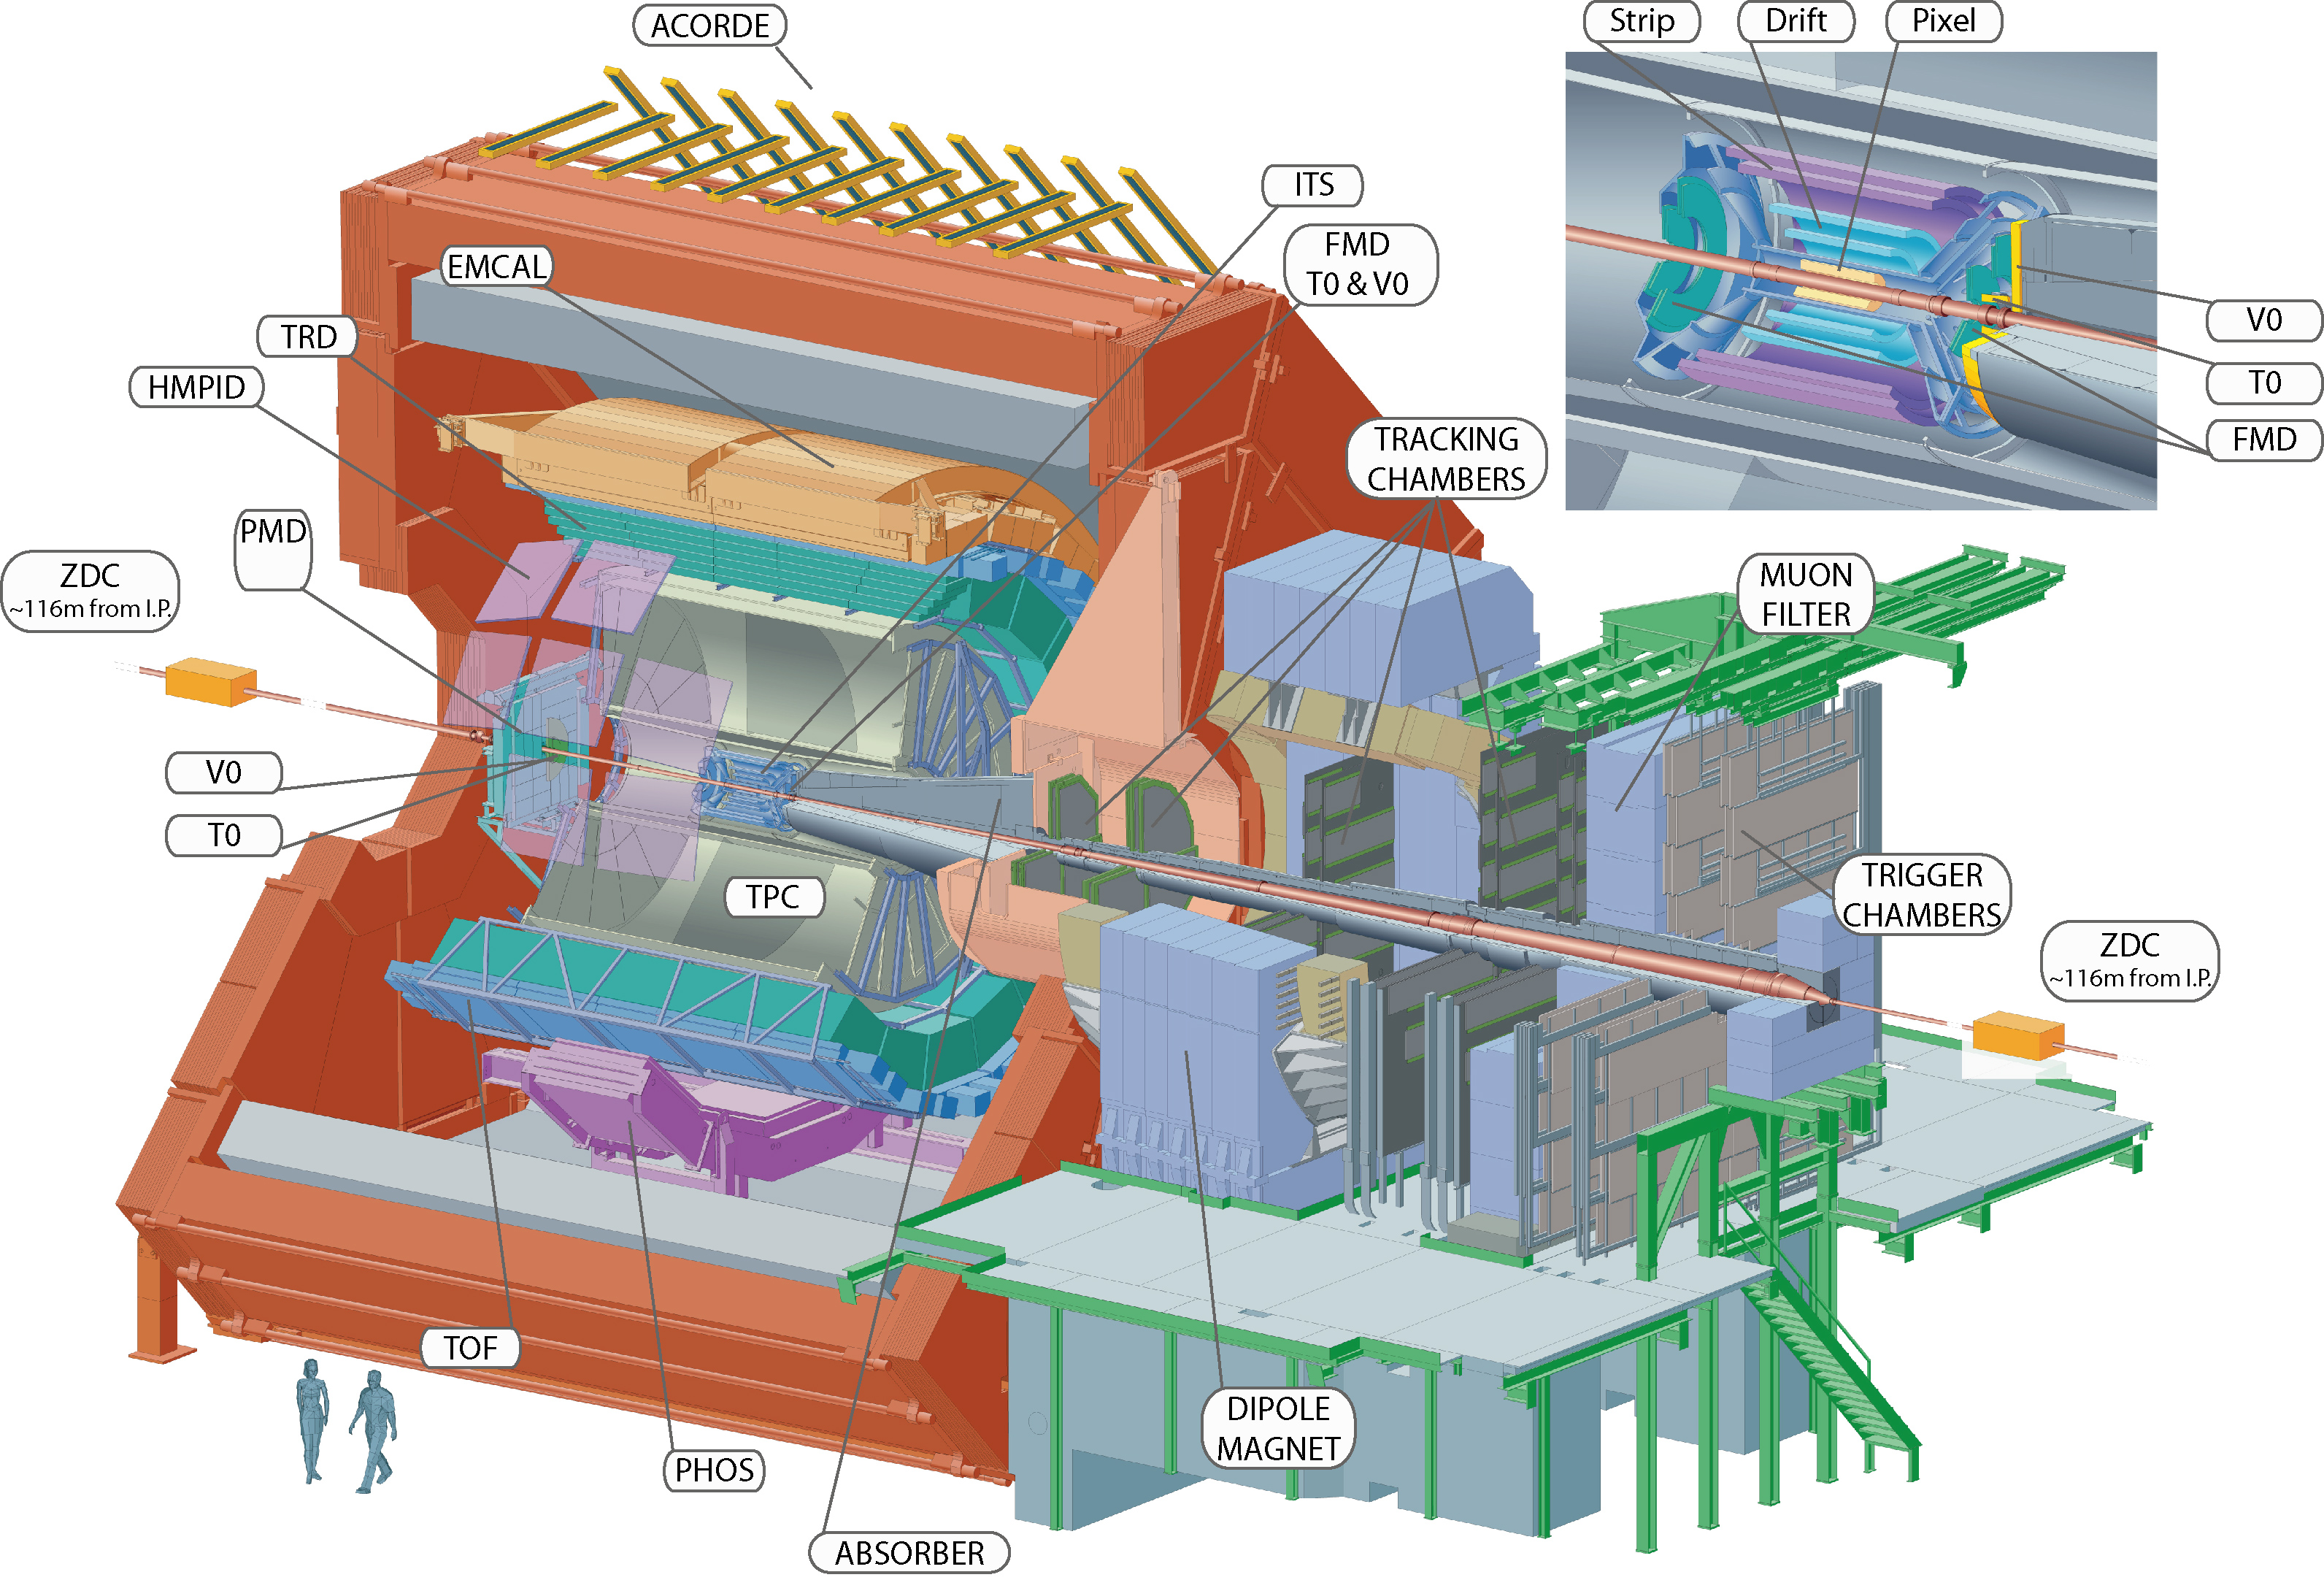
\includegraphics[width=\textwidth]{img/ALICE_Schematics}

\column{.42\textwidth}
\begin{itemize}
\item Important features
\begin{itemize}
\item \alert{PID} \\
(e, $\mu$, $\pi$, K, p, d, ${}^3$He)
\item \alert{low-momentum tracking} ($\pt > 0.15$~\GeVc)
\end{itemize}
\item \alert{D mesons} via hadronic decays (ITS, TPC, TOF)
\begin{itemize}
\item PID, topological cuts
\item invariant mass analysis
\end{itemize}
\end{itemize}
\end{columns}
\begin{itemize}
\item \alert{Jet reconstruction} using \antikt\ algorithm
\begin{itemize}
\item \textcolor{ForestGreen}{charged constituents} (ITS, TPC) $\rightarrow$ \emph{charged jets} (this analysis)
\item add \textcolor{NavyBlue}{neutral constituents} (EMCal, DCal) $\rightarrow$ \emph{full jets} 
\end{itemize}
\end{itemize}
\end{frame}

\begin{frame}[t]{Jet Energy Scale shift and \pt\ resolution}
\begin{columns}
\column{.47\textwidth}
\begin{overpic}[width=\textwidth]{img/ALICE_JetRes}
\put (-3,4) {{\tiny PRD 91 (2015) 112012}}
\end{overpic}\\
\medskip
{\small
\textcolor{BrickRed}{
\textbf{Inclusive Charged Jets} \\
\medskip
$\mu [(\ptchjetdet-\ptchjetgen)/\ptchjetgen]\approx -3\%$ \\
\smallskip
$\sigma[(\ptchjetdet-\ptchjetgen)/\ptchjetgen]\approx17\%$
}}
\column{.53\textwidth}
\medskip
\begin{overpic}[width=\textwidth, trim=0 0 30 22, clip]{img/HQ16_Simulation_DetectorResponse}
\end{overpic}\\
\raggedleft
{\small
\textcolor{NavyBlue}{
\textbf{D-Tagged Charged Jets}\\
\medskip
$\mu[(\ptchjetdet-\ptchjetgen)/\ptchjetgen]\approx -3\%$ \\
\smallskip
$\sigma[(\ptchjetdet-\ptchjetgen)/\ptchjetgen]\approx11\%$
}}
\end{columns}
\bigskip
\centering
\textbf{slightly better \ptchjet\ resolution due to the D-meson requirement}
\end{frame}

\begin{frame}[t]{Signal extraction}
\begin{columns}[T]
\column{.5\textwidth}
\begin{overpic}[width=\textwidth, trim=0 0 0 50, clip]{img/HQ16_Simulation_InvMass}
\end{overpic}
\column{.5\textwidth}
\textbf{\alert{Three methods}}
\begin{enumerate}
\item \textcolor{BrickRed}{Side-Band (S-B) background subtraction}
\item \textcolor{ForestGreen}{Like-Sign (L-S) background subtraction}
\item \textcolor{NavyBlue}{Invariant Mass fit in bins of \ptchjet}
\end{enumerate}
\end{columns}
\end{frame}

\begin{frame}[t]{Signal extraction: S-B method}
\begin{columns}[T]
\column{.50\textwidth}
\begin{overpic}[width=\textwidth, trim=0 0 0 50, clip]{img/HQ16_Simulation_InvMass}
\end{overpic}
\column{.50\textwidth}
\textbf{\textcolor{BrickRed}{Method 1: Side-Band (S-B)}}
\begin{enumerate}
\item Fill D-meson invariant mass distributions in bins of \alert{\ptd}
\item $N(\ptchjet, \ptd)$ distributions in\\
\medskip
\textcolor{NavyBlue}{\textbf{Peak Area}\\
{\scriptsize $|M_{\rm K\pi} - M_{\rm fit}| <2\sigma_{\rm fit}$}\\ 
\smallskip
$N_{\rm sig+bkg} (\ptchjet, \ptd)$}\\
\medskip
\textcolor{BrickRed}{\textbf{Side Bands}\\
{\scriptsize $8\sigma_{\rm fit} <|M_{\rm K\pi} - M_{\rm fit}| < 4\sigma_{\rm fit}$}\\ 
\smallskip
$N_{\rm bkg, SB} (\ptchjet, \ptd)$}
\end{enumerate}
\end{columns}
\begin{enumerate}
\setcounter{enumi}{2}
\item Apply \textcolor{VioletRed}{efficiency correction} and \textcolor{YellowOrange}{integrate in \ptd}
{\small $$N_{\rm signal} (\ptchjet)=\textcolor{YellowOrange}{\sum_{\ptd}} \textcolor{VioletRed}{\frac{1}{\epsilon(\ptd)}} [\textcolor{NavyBlue}{N_{\rm sig+bkg}(\ptchjet, \ptd)} - \frac{B^{*}}{B}\textcolor{BrickRed}{N_{\rm bkg,SB}(\ptchjet, \ptd)}]$$}
\end{enumerate}
\end{frame}

\begin{frame}[t]{Signal extraction: L-S method}
\begin{columns}[T]
\column{.50\textwidth}
\begin{overpic}[width=\textwidth, trim=0 0 0 50, clip]{img/HQ16_Simulation_InvMass}
\end{overpic}
\column{.50\textwidth}
\textbf{\textcolor{ForestGreen}{Method 2: Like-Sign (L-S)}}
\begin{enumerate}
\item Fill D-meson invariant mass distributions in bins of \alert{\ptd}
\item $N(\ptchjet, \ptd)$ distributions in\\
\medskip
\textcolor{NavyBlue}{\textbf{U-S peak area}\\
{\scriptsize $|M_{\rm K\pi} - M_{\rm fit}| <2\sigma_{\rm fit}$}\\ 
\smallskip
{\small $N_{\rm sig+bkg} (\ptchjet, \ptd)$}}\\
\medskip
\textcolor{ForestGreen}{\textbf{L-S peak area}\\
{\scriptsize $|M_{\rm K\pi} - M_{\rm fit}| <2\sigma_{\rm fit}$}\\ 
\smallskip
{\small $N_{\rm bkg, LS} (\ptchjet, \ptd)$}}
\end{enumerate}
\end{columns}
\begin{enumerate}
\setcounter{enumi}{2}
\item Apply \textcolor{VioletRed}{efficiency correction} and \textcolor{YellowOrange}{integrate in \ptd}
{\small $$N_{\rm signal} (\ptchjet)=\textcolor{YellowOrange}{\sum_{\ptd}} \textcolor{VioletRed}{\frac{1}{\epsilon(\ptd)}} [\textcolor{NavyBlue}{N_{\rm sig+bkg}(\ptchjet, \ptd)} - \frac{B^{*}}{B}\textcolor{ForestGreen}{N_{\rm bkg,LS}(\ptchjet, \ptd)}]$$}
\end{enumerate}
\end{frame}

\begin{frame}[t]{Signal extraction: invariant mass fit}
\begin{columns}[T]
\column{.5\textwidth}
\begin{overpic}[width=\textwidth, trim=0 0 0 50, clip]{img/HQ16_Simulation_InvMass}
\end{overpic}
\column{.5\textwidth}
\textbf{\textcolor{NavyBlue}{Method 3: invariant mass fit}}
\begin{enumerate}
\item Fill D-meson invariant mass distributions in bins of \alert{\ptchjet}
\item \textbf{Fit invariant mass distributions} with a \\ Gaussian (\textcolor{NavyBlue}{signal}) + exponential (\textcolor{BrickRed}{background})
\item Extract $N_{\rm signal} (\ptchjet)$ from fit parameters
\end{enumerate}
\end{columns}
\begin{itemize}
\item The correction for the D-tagged jet reconstruction efficiency must be applied as a weight when filling the invariant mass plots
\end{itemize}
\end{frame}

\begin{frame}{Raw Signal Extraction (Monte Carlo)}
\begin{columns}
\column{.55\textwidth}
\begin{overpic}[width=\textwidth, trim=0 0 50 0, clip]{img/HQ16_Simulation_MethodComparison}
\end{overpic}
\column{.45\textwidth}
\begin{itemize}
\item PYTHIA6 Perugia-2011 and GEANT3
\medskip
\item D-tagged jet signal yields extracted using the  \textbf{\textcolor{NavyBlue}{invariant mass fit}}, \textbf{\textcolor{BrickRed}{Side-Band}} 
and \textbf{\textcolor{ForestGreen}{Like-Sign}} methods are compared with the \textbf{\textcolor{gray}{MC truth}}
\medskip
\item All methods \textbf{agree well} with the MC truth within their statistical uncertainties
\end{itemize}
\end{columns}
\end{frame}

\end{document}
